% ============================================================================
% Apêndices (incluídos por resultados_preliminares_pgc3.tex)
% ============================================================================
\chapter{Reprodutibilidade}
\label{ap:repro}

Os comandos a seguir, executados a partir da raiz do repositório em
PowerShell, reproduzem os resultados, executam os testes e compilam este
documento. A base legada não acompanha o repositório: o caminho do arquivo
\arq{Data.zip}, ou da pasta \arq{Data/Data}, é informado pela opção
\texttt{--data} ou pela variável de ambiente \texttt{IRIS\_LEGACY\_DATA}.

\begin{SingleSpace}
\footnotesize
\begin{verbatim}
$env:IRIS_LEGACY_DATA = "C:\caminho\para\Data.zip"
.\.venv\Scripts\python.exe experiments\pgc3_vascular_pipeline.py
.\.venv\Scripts\python.exe experiments\pgc3_pupil_geometry.py
.\.venv\Scripts\python.exe experiments\pgc3_numbers.py
.\.venv\Scripts\python.exe -m unittest discover -s tests
cd docs\PGC_3
pdflatex resultados_preliminares_pgc3.tex
pdflatex resultados_preliminares_pgc3.tex
\end{verbatim}
\end{SingleSpace}

O primeiro \emph{script} levou \val{tempo-a} minutos e o segundo,
\val{tempo-b} minutos, numa máquina com \val{env-cpus} processadores lógicos.
As features de cada representação ficam guardadas em
\arq{results/pgc3/cache}, de modo que execuções seguintes reaproveitam a
extração. As partições da validação cruzada usam as sementes 2026 a 2035; o
teste de permutação, as sementes 10000 a 10999; e a coorte sintética,
sementes fixas por olho. O ambiente usou Python \val{env-python}, NumPy
\val{env-numpy}, SciPy \val{env-scipy}, scikit-learn \val{env-sklearn}
\citep*{Pedregosa2011}, scikit-image \val{env-skimage} \citep*{vanderWalt2014}
e OpenCV \val{env-opencv} \citep*{Bradski2000}.

Os testes automatizados (\arq{tests/test_pgc3.py}) verificam o bloqueio de
objetos arbitrários na leitura dos arquivos legados, a remoção de cópias, o
reparo da costura e a detecção de faixas espelhadas; o ajuste de Holm, o
alargamento do intervalo pela correção de Nadeau e Bengio e os postos de
Friedman; a exatidão da inversa da normalização (Equação~\ref{eq:inversa}) e
a invariância da faixa à dilatação; a medição de $\rho$ em olhos sintéticos
com erro menor que 0,01; a recuperação do sinal geométrico pela fusão; a
compatibilidade do AdaBoost com as versões recentes do scikit-learn; e a
leitura sem cópias pelo pipeline da IC.

% ----------------------------------------------------------------------------
\chapter{Tabelas completas da grade}
\label{ap:tabelas}

As Tabelas~\ref{tab:gradepixels} a \ref{tab:gradeic} trazem a acurácia
balanceada e, entre parênteses, a AUC de cada configuração, em média de 50
\emph{folds}; o negrito indica a melhor representação de cada classificador.
A Tabela~\ref{tab:resumo} resume as representações, e a
Tabela~\ref{tab:melhores} traz a melhor combinação de cada uma, com
intervalos de confiança corrigidos. Escolher a melhor entre 15 combinações é
uma seleção otimista; esses valores descrevem o teto observado nesta base e
não devem ser lidos como estimativas de desempenho.

\begin{table}[htbp]
  \centering
  \caption{Grade com o conjunto de pixels}
  \label{tab:gradepixels}
  \footnotesize
  \resizebox{\textwidth}{!}{% Gerado por experiments/pgc3_vascular_pipeline.py (não editar à mão).
\begin{tabular}{lccccc}
\toprule
Representação & RL & SVM & RF & MLP & AdaBoost \\
\midrule
Original (cinza) & 0,691 (0,772) & 0,655 (0,739) & 0,707 (0,776) & 0,745 (0,801) & 0,697 (0,765) \\
Equalização global & 0,755 (0,843) & 0,734 (0,831) & 0,743 (0,832) & 0,763 (0,841) & 0,705 (0,767) \\
CLAHE & 0,691 (0,775) & 0,700 (0,795) & 0,730 (0,798) & 0,736 (0,818) & 0,698 (0,772) \\
Verde + CLAHE & 0,708 (0,776) & 0,718 (0,806) & 0,707 (0,785) & 0,721 (0,787) & 0,698 (0,764) \\
\midrule
Frangi & 0,768 (0,812) & 0,724 (0,795) & 0,799 (0,843) & 0,769 (0,819) & \textbf{0,772 (0,834)} \\
Gabor & 0,766 (0,832) & 0,758 (0,836) & 0,769 (0,820) & 0,748 (0,817) & 0,706 (0,763) \\
\textit{Black-hat} & \textbf{0,779 (0,859)} & 0,763 (0,851) & 0,774 (0,852) & \textbf{0,798 (0,896)} & 0,751 (0,811) \\
Frangi + \textit{black-hat} & 0,751 (0,807) & \textbf{0,781 (0,816)} & \textbf{0,803 (0,854)} & 0,784 (0,847) & 0,743 (0,808) \\
\bottomrule
\end{tabular}
}
  \par\medskip
  \footnotesize Fonte: elaborada pelo autor.
\end{table}

\begin{table}[htbp]
  \centering
  \caption{Grade com o conjunto de textura}
  \label{tab:gradetextura}
  \footnotesize
  \resizebox{\textwidth}{!}{% Gerado por experiments/pgc3_vascular_pipeline.py (não editar à mão).
\begin{tabular}{lccccc}
\toprule
Representação & RL & SVM & RF & MLP & AdaBoost \\
\midrule
Original (cinza) & 0,821 (0,891) & \textbf{0,847 (0,880)} & \textbf{0,859 (0,908)} & 0,812 (0,902) & \textbf{0,854 (0,903)} \\
Equalização global & \textbf{0,822 (0,893)} & 0,840 (0,884) & 0,849 (0,883) & \textbf{0,871 (0,924)} & 0,806 (0,871) \\
CLAHE & 0,790 (0,875) & 0,823 (0,877) & 0,792 (0,863) & 0,826 (0,903) & 0,772 (0,851) \\
Verde + CLAHE & 0,756 (0,850) & 0,783 (0,861) & 0,746 (0,837) & 0,806 (0,882) & 0,739 (0,809) \\
\midrule
Frangi & 0,809 (0,861) & 0,783 (0,861) & 0,779 (0,839) & 0,761 (0,825) & 0,766 (0,829) \\
Gabor & 0,762 (0,813) & 0,800 (0,848) & 0,810 (0,858) & 0,773 (0,858) & 0,772 (0,826) \\
\textit{Black-hat} & 0,775 (0,851) & 0,793 (0,863) & 0,771 (0,850) & 0,810 (0,884) & 0,737 (0,800) \\
Frangi + \textit{black-hat} & 0,763 (0,833) & 0,776 (0,828) & 0,759 (0,824) & 0,748 (0,809) & 0,743 (0,798) \\
\bottomrule
\end{tabular}
}
  \par\medskip
  \footnotesize Fonte: elaborada pelo autor.
\end{table}

\begin{table}[htbp]
  \centering
  \caption{Grade com o conjunto padrão da IC}
  \label{tab:gradeic}
  \footnotesize
  \resizebox{\textwidth}{!}{% Gerado por experiments/pgc3_vascular_pipeline.py (não editar à mão).
\begin{tabular}{lccccc}
\toprule
Representação & RL & SVM & RF & MLP & AdaBoost \\
\midrule
Original (cinza) & 0,706 (0,799) & 0,677 (0,765) & 0,759 (0,830) & 0,756 (0,835) & \textbf{0,837 (0,910)} \\
Equalização global & 0,763 (0,855) & 0,741 (0,844) & 0,781 (0,869) & 0,758 (0,849) & 0,806 (0,872) \\
CLAHE & 0,698 (0,787) & 0,708 (0,804) & 0,727 (0,804) & 0,751 (0,832) & 0,746 (0,829) \\
Verde + CLAHE & 0,720 (0,786) & 0,721 (0,813) & 0,713 (0,800) & 0,726 (0,799) & 0,719 (0,801) \\
\midrule
Frangi & 0,775 (0,820) & 0,726 (0,801) & 0,799 (0,852) & 0,769 (0,818) & 0,769 (0,830) \\
Gabor & 0,767 (0,834) & 0,770 (0,838) & 0,785 (0,840) & 0,752 (0,812) & 0,759 (0,807) \\
\textit{Black-hat} & \textbf{0,786 (0,863)} & 0,766 (0,852) & 0,776 (0,855) & \textbf{0,802 (0,898)} & 0,745 (0,811) \\
Frangi + \textit{black-hat} & 0,755 (0,812) & \textbf{0,783 (0,818)} & \textbf{0,810 (0,845)} & 0,763 (0,830) & 0,751 (0,806) \\
\bottomrule
\end{tabular}
}
  \par\medskip
  \footnotesize Fonte: elaborada pelo autor.
\end{table}

\begin{table}[htbp]
  \centering
  \caption{Resumo por representação: médias da grade, postos de Friedman,
  comparações com a original e teste de permutação}
  \label{tab:resumo}
  \footnotesize
  \resizebox{\textwidth}{!}{% Gerado por experiments/pgc3_vascular_pipeline.py (não editar à mão).
\begin{tabular}{lccccccc}
\toprule
\multirow{2}{*}{Representação} & \multicolumn{2}{c}{Média da grade} & \multicolumn{2}{c}{Posto médio} & \multicolumn{2}{c}{vs.\ original (Holm)} & Permutação \\
\cmidrule(lr){2-3}\cmidrule(lr){4-5}\cmidrule(lr){6-7}
 & AB & AUC & AB & AUC & $\uparrow$ / $\downarrow$ & $\Delta$AB médio & $p$ \\
\midrule
Original (cinza) & 0,762 & 0,832 & 4,87 & 4,67 & -- & -- & $<$0,001 \\
Equalização global & 0,782 & 0,857 & 3,20 & 2,20 & 0 / 0 & $+$0,021 & $<$0,001 \\
CLAHE & 0,746 & 0,826 & 5,73 & 4,73 & 0 / 0 & $-$0,016 & $<$0,001 \\
Verde + CLAHE & 0,732 & 0,810 & 6,87 & 6,67 & 0 / 0 & $-$0,030 & $<$0,001 \\
\midrule
Frangi & 0,771 & 0,829 & 3,60 & 4,47 & 0 / 0 & $+$0,010 & $<$0,001 \\
Gabor & 0,766 & 0,827 & 4,00 & 5,20 & 0 / 0 & $+$0,005 & $<$0,001 \\
\textit{Black-hat} & 0,775 & 0,853 & 3,60 & 2,80 & 0 / 0 & $+$0,013 & $<$0,001 \\
Frangi + \textit{black-hat} & 0,767 & 0,822 & 4,13 & 5,27 & 0 / 0 & $+$0,006 & $<$0,001 \\
\bottomrule
\end{tabular}
}
  \par\medskip
  \footnotesize Fonte: elaborada pelo autor. AB: acurácia balanceada;
  $\uparrow$/$\downarrow$: combinações significativamente melhores ou piores
  que a original após o ajuste de Holm sobre as 105 comparações; permutação:
  RL sobre os pixels.
\end{table}

\begin{table}[htbp]
  \centering
  \caption{Melhor combinação de cada representação (seleção otimista)}
  \label{tab:melhores}
  \footnotesize
  \resizebox{\textwidth}{!}{% Gerado por experiments/pgc3_vascular_pipeline.py (não editar à mão).
\begin{tabular}{llcccc}
\toprule
Representação & Combinação & AB [IC 95\%] & AUC [IC 95\%] & Sensib. & Especif. \\
\midrule
Original (cinza) & Textura + RF & 0,859 [0,773; 0,946] & 0,908 [0,834; 0,981] & 0,819 & 0,899 \\
Equalização global & Textura + MLP & 0,871 [0,805; 0,936] & 0,924 [0,866; 0,982] & 0,837 & 0,905 \\
CLAHE & Textura + MLP & 0,826 [0,750; 0,902] & 0,903 [0,845; 0,962] & 0,794 & 0,857 \\
Verde + CLAHE & Textura + MLP & 0,806 [0,726; 0,887] & 0,882 [0,814; 0,949] & 0,778 & 0,834 \\
\midrule
Frangi & Textura + RL & 0,809 [0,733; 0,884] & 0,861 [0,784; 0,937] & 0,755 & 0,862 \\
Gabor & Textura + RF & 0,810 [0,725; 0,895] & 0,858 [0,774; 0,943] & 0,770 & 0,849 \\
\textit{Black-hat} & Textura + MLP & 0,810 [0,726; 0,894] & 0,884 [0,814; 0,955] & 0,794 & 0,826 \\
Frangi + \textit{black-hat} & Padrão da IC + RF & 0,810 [0,744; 0,876] & 0,845 [0,768; 0,923] & 0,714 & 0,906 \\
\bottomrule
\end{tabular}
}
  \par\medskip
  \footnotesize Fonte: elaborada pelo autor.
\end{table}

\begin{table}[htbp]
  \centering
  \caption{Replicação no leiaute \texttt{personBase}: diferença de acurácia
  balanceada em relação à original e valor $p$ ajustado por Holm}
  \label{tab:efeitopb}
  \footnotesize
  % Gerado por experiments/pgc3_vascular_pipeline.py (não editar à mão).
\begin{tabular}{lccc}
\toprule
Representação & Pixels & Textura & Padrão da IC \\
\midrule
Equalização global & $+$0,003 (1,000) & $-$0,002 (0,917) & $-$0,004 (1,000) \\
CLAHE & $-$0,013 (1,000) & $-$0,023 (0,601) & $-$0,023 (1,000) \\
Verde + CLAHE & $-$0,004 (1,000) & $-$0,042 (0,090) & $-$0,022 (1,000) \\
\midrule
Frangi & $+$0,008 (1,000) & $-$0,039 (0,601) & $-$0,013 (1,000) \\
Gabor & $+$0,026 (1,000) & $-$0,047 (0,372) & $+$0,006 (1,000) \\
\textit{Black-hat} & $-$0,007 (1,000) & $-$0,036 (0,601) & $-$0,034 (1,000) \\
Frangi + \textit{black-hat} & $-$0,006 (1,000) & $-$0,030 (0,601) & $-$0,025 (1,000) \\
\bottomrule
\end{tabular}

  \par\medskip
  \footnotesize Fonte: elaborada pelo autor.
\end{table}

A Figura~\ref{fig:roc} mostra as curvas ROC médias de cada representação no
leiaute principal, para o modelo pré-especificado (RL com o conjunto padrão da
IC) e para a melhor combinação de cada representação, e a
Figura~\ref{fig:cdauc} repete o ranking de Friedman com a AUC.

\begin{figure}[htbp]
  \centering
  \caption{Curvas ROC médias por representação (\texttt{personBase\_invert})}
  \label{fig:roc}
  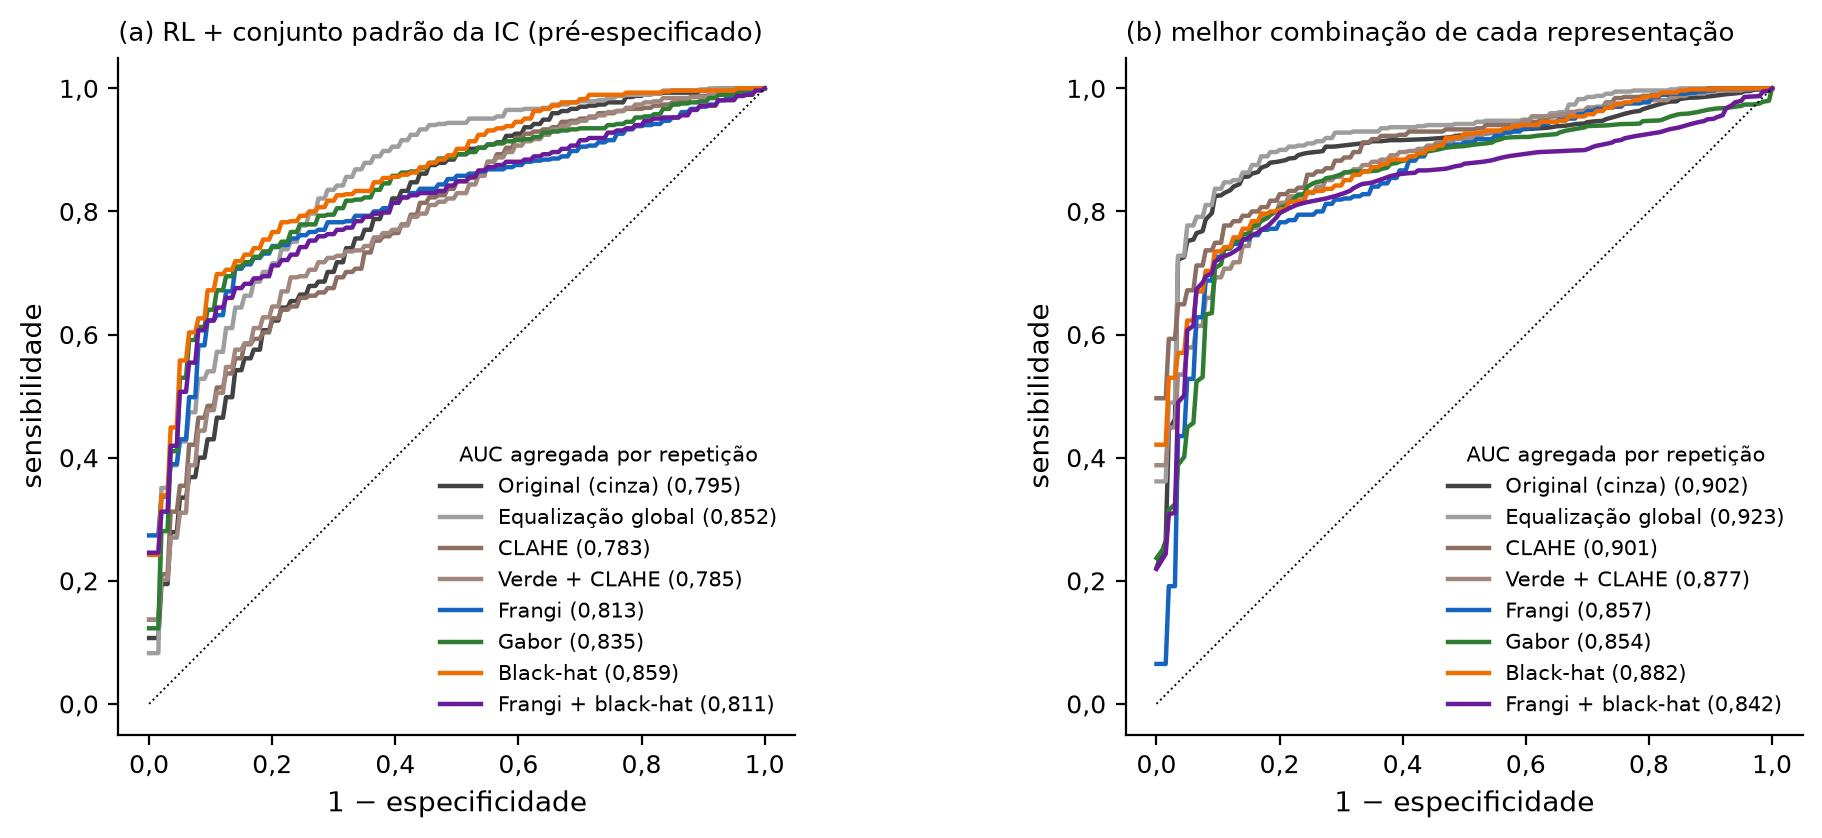
\includegraphics[width=\textwidth]{roc_representacoes.png}
  \par\medskip
  \footnotesize Fonte: elaborada pelo autor. Escores fora do \emph{fold}
  agregados por repetição; o painel (b) resulta de uma seleção otimista.
\end{figure}

\begin{figure}[htbp]
  \centering
  \caption{Postos médios de Friedman pela AUC e diferença crítica de Nemenyi}
  \label{fig:cdauc}
  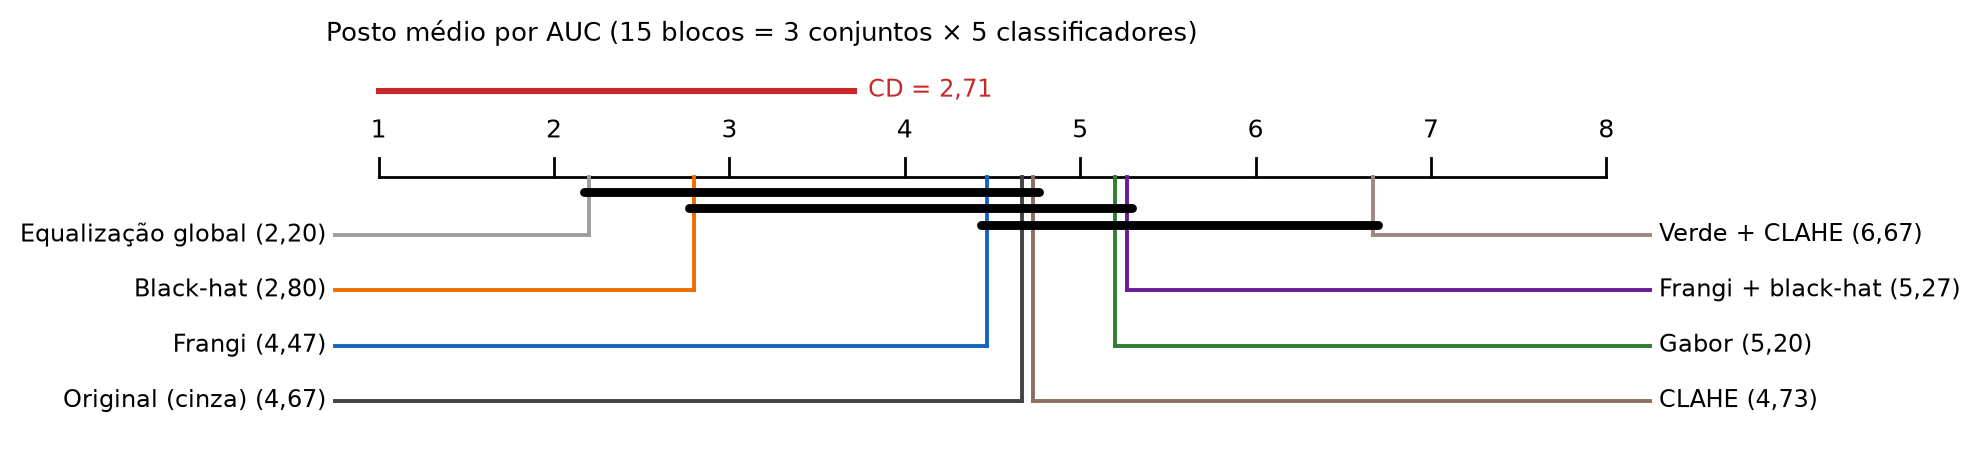
\includegraphics[width=0.95\textwidth]{diferenca_critica_auc.png}
  \par\medskip
  \footnotesize Fonte: elaborada pelo autor.
\end{figure}

% ----------------------------------------------------------------------------
\chapter{Parâmetros}
\label{ap:parametros}

\begin{quadro}[htb]
  \caption{Parâmetros dos realces, dos descritores e dos experimentos}
  \label{qua:parametros}
  \footnotesize
  \begin{tabular}{p{4.4cm}p{9.8cm}}
    \toprule
    Componente & Valores \\
    \midrule
    CLAHE & limite de contraste 2,0; grade de $8\times8$ \\
    Frangi & $\sigma\in\{1,2,3,4\}$; $\beta=0{,}5$; $c=15$; cristas claras;
      exibição por percentis 2 e 99 com gama 0,7 \\
    Gabor & 8 orientações; núcleo $21\times21$; $\sigma=4$;
      $\lambda=10$; $\gamma=0{,}5$; média do núcleo removida \\
    Morfologia & \tht{} e \bh{} com elementos elípticos de 5, 11 e 21 pixels \\
    Pixels & subamostragem por 4 com suavização ($50\times180$) \\
    LBP & uniforme, 16 vizinhos, raio 2, histograma de 18 posições \\
    GLCM & 64 níveis; distâncias 1, 2 e 3; ângulos 0°, 45°, 90° e 135°;
      contraste, dissimilaridade, homogeneidade, energia, correlação e ASM \\
    Estatísticas de intensidade & média, desvio-padrão, assimetria, curtose e
      histograma de 32 posições \\
    Classificadores & RL ($C=1$); SVM RBF ($C=1$, $\gamma$ automático); RF
      (100 árvores); MLP (100 e 50 neurônios, Adam); AdaBoost (50
      estimadores); semente 42 \\
    Validação cruzada & estratificada por grupos, 5 \emph{folds}, 10
      repetições (sementes 2026 a 2035) \\
    Permutação & RL sobre pixels; 5 \emph{folds}; 1000 permutações \\
    Detector de pupila & 72 raios; pico a 30\% do máximo do raio; RANSAC com
      tolerância de 2 pixels; refinamento integro-diferencial com $\sigma=1{,}5$
      e primeiro pico a 50\% \\
    Detector de limbo & arcos laterais de $-45$° a 45° e de 135° a 225°;
      RANSAC com tolerância de 3 pixels \\
    Coorte sintética & imagens de $480\times480$; raio da íris entre 29\% e 35\%
      do lado; excentricidade de até 0,04; ruído com desvio de 1,5 a 4,5 \\
    \bottomrule
  \end{tabular}
  \par\medskip
  \footnotesize Fonte: elaborado pelo autor.
\end{quadro}
